%____________________WEEK 2_____________________________%
\newpage
\section{Tuần 2}
\subsection{Quy trình xây dựng chương trình AI}

\subsection{Tiền xử lý (Data preprocessing)}
- Dữ liệu được tiền xử lý bằng cách:
\\- Sau khi tiền xử lý, dữ liệu được chia ra cho các bước tiếp theo bằng cách:
\subsection{Huấn luyện mô hình (Train model/Tune model)}
- Mô hình dự đoán 1 mẫu ntn? VD?
\\- Activation function, chức năng, VD
\\- Loss function, chức năng, VD
\\- Optimizer, thuật toán chủ đạo của Optimizer, cách thuật toán hoạt động.
\subsubsection{Cách mô hình dự đoán}
\subsubsection{Activation function}
\subsubsection{Loss function}
\subsubsection{Optimizer}
\subsection{Đánh giá mô hình (Test model)}
- Đo lường hiệu suất để đánh giá mô hình là một phần trong quy trình xây dựng máy học. Tất cả các mô hình máy học đều cần \textbf{metric} để đánh giá hiệu suất.
\\- Với \textbf{supervised learning}, có 2 bài toán lớn là \textbf{Regression} và \textbf{Classification}. Sau đây là các \textbf{metric} phổ biến đối với 2 bài toán này: \footnote{Các metric phổ biến dùng trong test model. Cách tính, ý nghĩa từng metric}
\subsubsection{Regression metrics}
Mô hình Regression có đầu ra liên tục (continuous output). Do đó, chúng ta cần một metric dựa trên việc tính toán khoảng cách giữa \textbf{giá trị được dự đoán} (predicted) và \textbf{giá trị thực tế} (ground truth). Các regression metric chủ yếu: \cite{lecture_og}
\begin{itemize}
    \item Mean Absolute Error (MAE)
    \item Mean Squared Error (MSE)
    \item Root Mean Squared Error (RMSE)
\end{itemize}

\begin{enumerate}

\item \textbf{Mean Absolute Error (MAE)} 
\begin{itemize}
\item Giá trị chênh lệch trung bình giữa giá trị thực tế và giá trị được dự đoán bởi mô hình Regression.

\begin{center}
\large $MAE = \frac{1}{N}\sum_{j=1}^{N}\left| y_{i}-\hat{y_{i}} \right|$
\end{center}
Trong đó:
\begin{itemize}
    \item $y_{i}$: giá trị thực tế
    \item $\hat{y_{i}}$: giá trị được dự đoán bởi mô hình Regression
    \item N: số lượng dữ liệu
\end{itemize}
\item Ý nghĩa :
\begin{itemize}
\item MAE có miền giá trị từ $[0,+\infty ]$. 
\item Trên cùng tập dữ liệu, MAE càng nhỏ thì có độ chính xác càng cao.
\item MAE không nhạy cảm với giá trị ngoại lệ (outliers) do việc sử dụng giá trị tuyệt đối.
\item MAE không phản ánh mức độ sai số cụ thể của mô hình. Nó không phân biệt được các lỗi dương và âm, chỉ cho ta biết lỗi trung bình.
\end{itemize}
\end{itemize}
\item\textbf{Mean Squared Error (MSE)}
\begin{itemize}

\item Giá trị trung bình của bình phương độ chênh lệch giữa giá trị mục tiêu và giá trị được dự đoán bởi mô hình Regression.

\begin{center}
\large $MSE = \frac{1}{N}\sum_{j=1}^{N}(y_{i}-\hat{y_{i}})^2$
\end{center}

Trong đó:
\begin{itemize}
    \item $y_{i}$: giá trị thực tế
    \item $\hat{y_{i}}$: giá trị được dự đoán bởi mô hình Regression
    \item N: số lượng dữ liệu
\end{itemize}
\item Ý nghĩa:
\begin{itemize}
\item MSE có miền giá trị từ $[0,+\infty ]$. 
\item Trên cùng tập dữ liệu, MSE càng nhỏ thì có độ chính xác càng cao. 
\item Vì lấy bình phương sai số nên đơn vị của MSE khác với đơn vị của kết quả dự đoán.
\item MSE nhạy cảm với các giá trị ngoại lệ (outliers) do tính bình phương. Các giá trị lớn hơn sẽ có ảnh hưởng lớn hơn đến MSE
\end{itemize}
\end{itemize}

\item \textbf{Root Mean Squared Error (RMSE)}
\begin{itemize}
\item Căn bậc hai giá trị trung bình của bình phương độ chênh lệch giữa giá trị mục tiêu và giá trị được dự đoán bởi mô hình Regression.
\begin{center}
\large $RMSE = \sqrt{\frac{1}{N}\sum_{j=1}^{N}(y_{i}-\hat{y_{i}})^2}$
\end{center}
Trong đó:
\begin{itemize}
    
    \item $y_{i}$: giá trị thực tế
    \item $\hat{y_{i}}$: giá trị được dự đoán bởi mô hình Regression
    \item N: số lượng dữ liệu
\end{itemize}
\item Ý nghĩa:
\begin{itemize}
\item RMSE có miền giá trị từ $[0,+\infty ]$. 
\item Trên cùng tập dữ liệu, RMSE càng nhỏ thì có độ chính xác càng cao. 
\item Việc lấy căn bậc 2 giúp RMSE có cùng đơn vị với kết quả dự đoán, đồng thời làm giá trị RMSE không quá lớn khi số lượng điểm dữ liệu lớn.
\item RMSE cũng như MSE, nhạy cảm với các giá trị ngoại lệ (outliers) do tính bình phương.
\end{itemize}
\end{itemize}

\end{enumerate}

\subsubsection{Classification metrics}
Các mô hình classification có \textbf{đầu ra rời rạc} (discrete output), vì vậy chúng ta cần metric so sánh các lớp rời rạc dưới một dạng nào đó.\\
Các classification metric đều đánh giá hiệu suất của mô hình và cho biết mức độ phân loại tốt hay xấu, nhưng mỗi metric lại đánh giá mô hình theo một cách khác nhau.\\
Các classification metric chủ yếu:
\begin{itemize}
    \item Accuracy
    \item Precision and Recall
    \item F1-score
    \item AU-ROC
\end{itemize}

\textbf{Confusion matrix} \cite{mlwiki} \cite{aiuit} là một kỹ thuật đánh giá hiệu năng của mô hình cho các bài toán phân lớp. Confusion matrix là một ma trận thể hiện số lượng điểm dữ liệu thuộc vào một class và được dự đoán thuộc vào class.\\
\textbf{Confusion matrix} cung cấp thêm thông tin về tỉ lệ phân lớp đúng giữa các lớp, hay giúp phát hiện các lớp có tỉ lệ phân lớp nhầm cao nhờ vào các khái niệm True (False) Positive (Negative)\\

\begin{figure}[H]
    \centering
    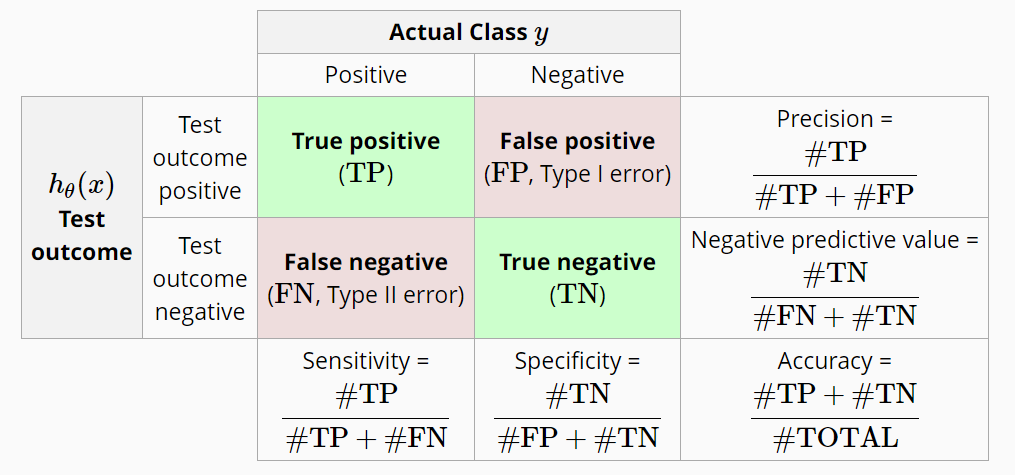
\includegraphics[width=1\linewidth]{img/binary_classifiers.png}
\end{figure}

\begin{itemize}
\item \textbf{True positive (TP):} Đối tượng ở lớp Positive, mô hình phân đối tượng vào lớp Positive (dự đoán đúng).
\item \textbf{True negative (TN):} Đối tượng ở lớp Negative, mô hình phân đối tượng vào lớp Negative (dự đoán đúng).
\item \textbf{False positive (FP):} Đối tượng ở lớp Negative, mô hình phân đối tượng vào lớp Positive (dự đoán sai).
\item \textbf{False negative (FN):} Đối tượng ở lớp Positive, mô hình phân đối tượng vào lớp Negative (dự đoán sai).
\end{itemize}
\begin{enumerate}
    \item \textbf{Accuracy} \cite{accuracy} 
    \begin{itemize}
        \item Accuracy (độ chính xác) đánh giá mô hình thường xuyên dự đoán đúng đến mức nào. 
        \item Độ chính xác là tỉ lệ giữa số điểm dữ liệu được dự đoán đúng và tổng số điểm dữ liệu.
        \item Accuracy lộ rõ hạn chế khi được sử dụng trên bộ dữ liệu không cân bằng (imbalanced dataset). Mô hình có thể đạt accuracy cao khi phân loại dữ liệu vào các lớp đa số.
        \begin{center}
        \large $Accuracy = \frac{Number\ of\ correct\ predictions }{Total\ number\ of\ predictions}$
        \end{center}
        \begin{center}
        \large $Accuracy = \frac{TP + TN}{TP + TN + FP + FN}$
        \end{center}
    \end{itemize}
    
    \item \textbf{Precision} \cite{precision_recall} 
     \begin{itemize}
        \item \textbf{Precision} (Positive Predictive Value): (True Positives) / (All Positive Predictions)
        \begin{center}
        \large $P = Precision = \frac{TP}{TP + FP}$
        \end{center}
        \item Ý nghĩa: "Khi mô hình dự đoán một mẫu là Positive, thì có bao nhiêu tỉ lệ mẫu đó thực sự là Positive?" Nếu Precision cao, tức là tỷ lệ dự đoán Positive đúng của mô hình là cao, và mô hình có khả năng phân loại Positive tốt.
    \end{itemize}

    \item \textbf{Recall} \cite{precision_recall} 
    \begin{itemize}
        \item \textbf{Recall} (True Positive Rate): (True Positives) / (All Actual Positives)
        \begin{center}
        \large $R = Recall = \frac{TP}{TP + FN}$
        \end{center}
        \item Ý nghĩa: "Khi có một mẫu Positive, thì có bao nhiêu tỉ lệ mẫu đó được mô hình dự đoán đúng?" Nếu Recall cao, tức là mô hình có khả năng phát hiện các mẫu Positive tốt.
    \end{itemize}

    \item \textbf{F Measure} \cite{fmeasure}
    \begin{itemize}
        \item \textbf{F-score}: là phép đo đánh giá hiệu suất của mô hình bằng cách kết hợp giữa precision P và recall R
        \begin{center}
        \large $F_\beta = \frac{(\beta^{2} + 1)\times P \times R}{\beta^{2}\times P + R}$
        \end{center}
        \begin{itemize}
            \item Khi $\beta$ tiến đến 0, độ ảnh hưởng của P sẽ càng lớn.
            \item Khi $\beta$ tiến đến $\infty $, độ ảnh hưởng của R sẽ càng lớn.
            \item Ý nghĩa: Sử dụng cả Precision và Recall để đánh giá hiệu suất mô hình.
        \end{itemize}
        \item \textbf{$F_1$-score:} Khi $\beta = 1$, ta được $F_1$-score
        \begin{center}
        \large $F_1 = 2 \frac{P \times R}{P + R}$
        \end{center}
        \begin{itemize}
            \item $F_1$-score: là trung bình điều hòa của precision P và recall R
            \item Ý nghĩa: Precision và Recall có mức độ quan trọng tương đương và cần metric đánh giá hiệu suất tổng thể của mô hình phân loại.
        \end{itemize}
    \end{itemize}

        \item \textbf{ROC Curve, AUC} \cite{roc_auc}
    \begin{itemize}
        \item \textbf{ROC curve:} Đường cong ROC (Receiver Operating Characteristic curve) là biểu đồ hiển thị hiệu suất của mô hình classification ở tất cả các ngưỡng phân loại (classification thresholds). Đường cong này vẽ hai tham số: 
        \begin{enumerate}
            \item True Positive Rate (TPR) - hay còn được gọi là Recall:
            \begin{center}
             \large $TPR = \frac{TP}{TP + FN}$
            \end{center}
            \item False Positive Rate (FPR):
            \begin{center}
             \large $FPR = \frac{FP}{FP + TN}$
            \end{center}
        \end{enumerate}
        Đường cong ROC vẽ đồ thị TPR so với FPR ở các ngưỡng phân loại khác nhau. Việc giảm ngưỡng phân loại sẽ phân loại nhiều mục hơn thành Positive, do đó làm tăng cả kết quả False Positive và kết quả True Positives thực sự. Hình dưới đây cho thấy một đường cong ROC điển hình:
        \begin{figure}[H]
            \centering
            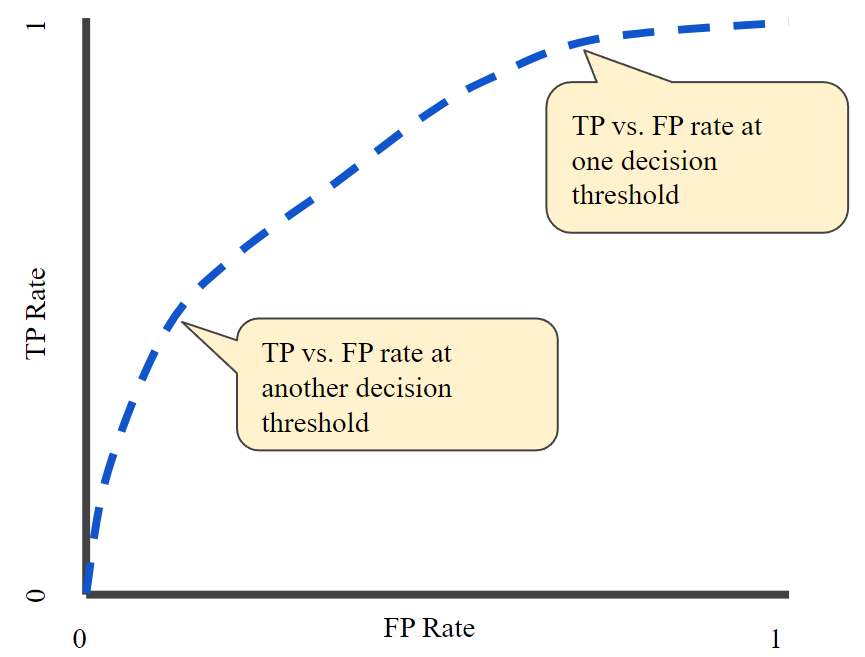
\includegraphics[width=0.5\linewidth]{img/ROC.png}
        \end{figure}
        \item \textbf{AUC:} Diện tích dưới đường cong ROC (Area Under the ROC Curve). AUC đo toàn bộ diện tích hai chiều bên dưới toàn bộ đường cong ROC từ (0,0) đến (1,1) - hay là phép tính tích phân của đường cong ROC từ 0 đến 1.
        \begin{center}
        \large $\int_{0}^{1} ROC(x)dx$
        \end{center}
        \begin{figure}[H]
            \centering
            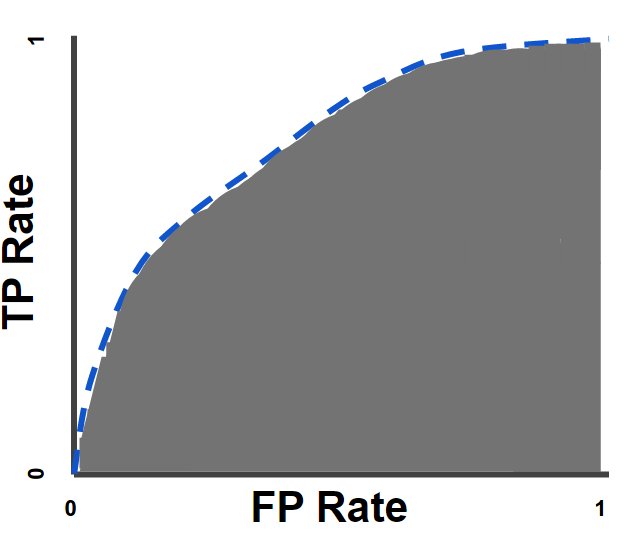
\includegraphics[width=0.5\linewidth]{img/AUC.png}
        \end{figure}
    \item \textbf{Ý nghĩa:} AUC có giá trị từ 0 đến 1. Với $AUC = 0$, mô hình dự đoán sai 100\%; với $AUC = 1$, mô hình dự đoán đúng 100\%.
    \begin{itemize}
        \item AUC không phụ thuộc vào tỷ lệ \textbf{(scale-invariant)}. AUC đo lường mức độ xếp hạng chính xác của các dự đoán, không phụ thuộc vào giá trị tuyệt đối của chúng.
        \item AUC không phụ thuộc vào ngưỡng phân loại \textbf{(classification-threshold-invariant)}. AUC đo lường chất lượng của các dự đoán mô hình bất kể ngưỡng phân loại được chọn
    \end{itemize}
    \end{itemize}
    
\end{enumerate}
